\chapter{Аналитическая часть}

В данном разделе будет проанализирована поставленная задача и рассмотрены различные способы ее реализации.

\section{Формализация задачи}

В ходе выполнения курсовой работы должно быть спроектировано и реализовано Web-приложение, позволяющее пользователю ознакомиться с прогнозами курса акций различных аналитиков. Пользователь должен иметь возможность получения прогнозируемой цены одной из предложенных акций. 
Кроме того, необходимо разработать ролевую модель, на основе которой будет строиться взаимодействие с веб-приложением. Предусмотреть три роли: пользователь, аналитик и администратор. Также необходимо создать систему регистрации и авторизации пользователей и предусмотреть возможность назначения ролей администратором. Сделать возможным для аналитика добавление, редактирование и удаление прогнозов.


\section{Формализация данных} 
База данных должна хранить информацию о:
\begin{itemize}
	\item компаниях;
 	\item прогнозах;
  \item финансовых показателях компаний;
  \item пользователях;
  \item действиях, совершаемых пользователями;
  \item группах пользователей;
  \item правах доступа пользователей.  
\end{itemize}


\begin{table}[H]
	\centering
	\caption{Категории данных и сведения о них}
	\label{tbl:categories}
	\resizebox{\textwidth}{!}{%
		\begin{tabular}{|l|l|}
			\hline
			\textbf{\begin{tabular}[c]{@{}c@{}}Категория\end{tabular}} & \textbf{Сведения}  \\ \hline
			Компания & ID компании, название, логотип, описание, тикер, ID показателей \\ \hline
			Прогноз & ID прогноза, инвест-дом, дата публикации, дата обновления, дата истечения, \\ & целевая цена, прогноз, описание прогноза, ID компании  \\ \hline
			Финансовые & ID показателей, цена, капитализация, объем прибыли до вычета налогов, \\ показатели & годовая выручка \\ \hline
			Пользователь & ID пользователя, имя пользователя в системе, пароль, \\  & электронная почта, полное имя \\ \hline
			Действия, совершаемые & ID записи, ID пользователя, ID группы пользователя,  \\ пользователями & информация об изменениях до и после \\ \hline
			Группа пользователей & ID записи, ID прав доступа, ID пользователя  \\ \hline
			Права доступа & ID записи, права доступа \\ \hline
		\end{tabular}%
	}
\end{table}


\section{Формализация ролей}
Должно быть выделено три категории пользователей.

\begin{table}[H]
	\centering
	\caption{Роли пользователей и предоставляемый им функционал}
	\label{tbl:roles_categories}
	\resizebox{\textwidth}{!}{%
		\begin{tabular}{|l|l|}
			\hline
			\textbf{\begin{tabular}[c]{@{}c@{}}Роль\end{tabular}} & \textbf{Функционал}  \\ \hline
			Пользователь & просмотр компаний и информации о них, \\ & просмотр прогнозов на выбранную компанию \\ \hline
			Аналитик & добавление, просмотр, редактирование, удаление компаний, информации о них, \\ & а также прогнозов на выбранную компанию \\ \hline
			Администратор & просмотр, добавление, редактирование, удаление выбранных пользователей \\ & и прав доступа \\ \hline
		\end{tabular}%
	}
\end{table}

\newpage
\section{Use-case диаграмма}

\begin{figure}[h!]
	\begin{center}
		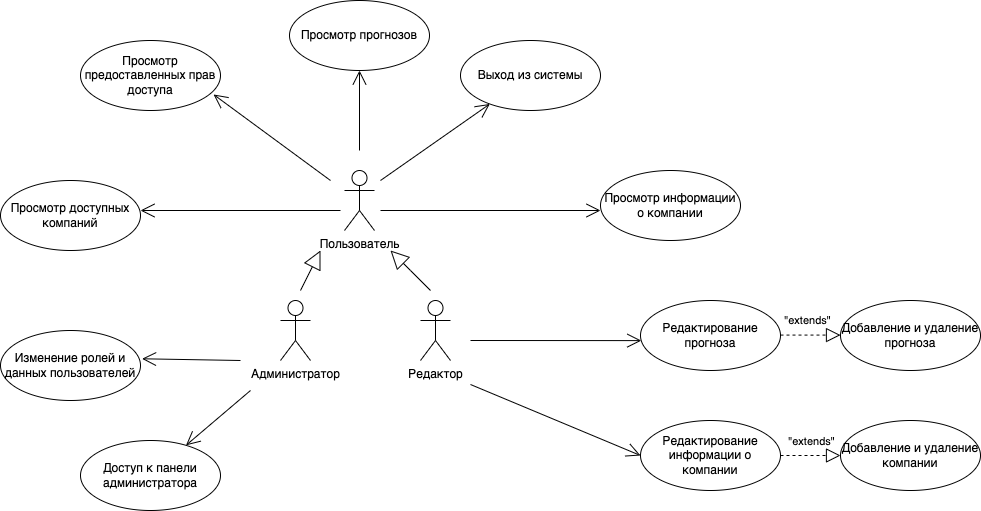
\includegraphics[scale=0.5]{img/use-case.png}
	\end{center}
	\captionsetup{justification=centering}
	\caption{Use-case диаграмма}
	\label{img:use-case}
\end{figure}

\newpage
\section{ER диаграмма}

\begin{figure}[h!]
	\begin{center}
		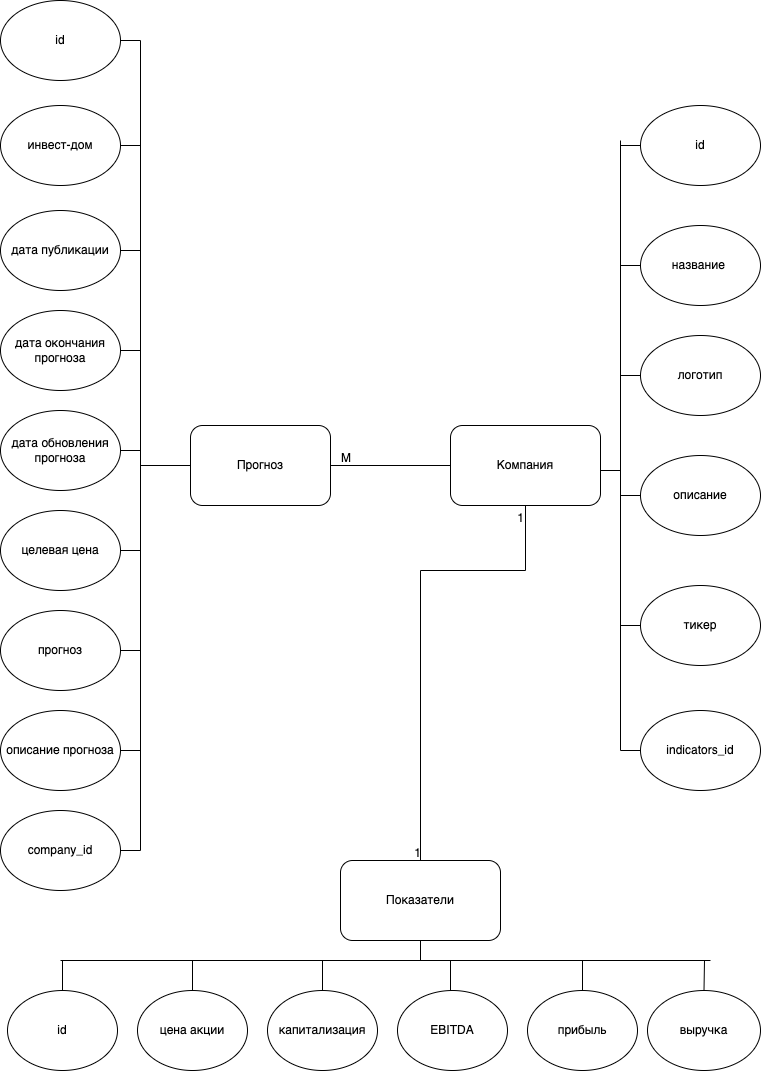
\includegraphics[scale=0.5]{img/er.drawio.png}
	\end{center}
	\captionsetup{justification=centering}
	\caption{ER диаграмма (1)}
	\label{img:er1}
\end{figure}
\newpage


\begin{figure}[h!]
	\begin{center}
		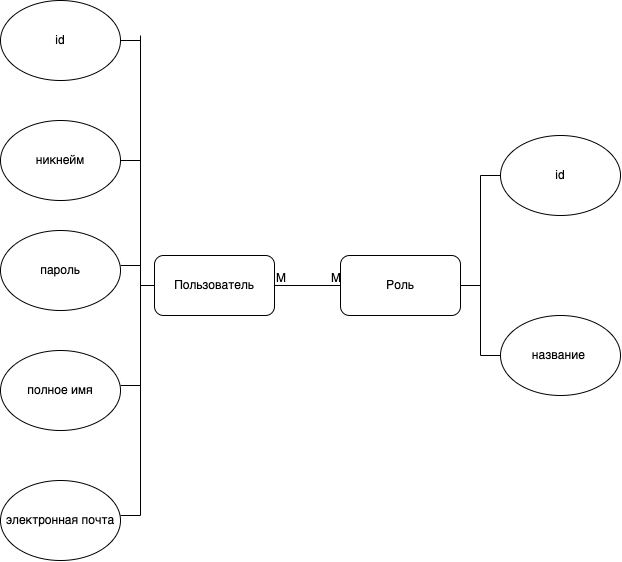
\includegraphics[scale=0.6]{img/er2.drawio.png}
	\end{center}
	\captionsetup{justification=centering}
	\caption{ER диаграмма (2)}
	\label{img:er2}
\end{figure}
\newpage


\section{Анализ существующих решений}
В качестве существующих решений для анализа выбраны сервисы Tinkoff Инвестиции, RBC Инвестиции, Investing.com, Finam.
В таблице \ref*{tbl:comparison} предствален сравнительный анализ существующих решений.

\begin{table}[H]
	\centering
	\caption{Анализ существующих решений}
	\label{tbl:comparison}
	\resizebox{\textwidth}{!}{%
		\begin{tabular}{|c|c|c|c|c|}
			\hline
			\textbf{Сервис} & \textbf{Деталиазация} & \textbf{Аргументация} & \textbf{Субъективность} & \textbf{Платный доступ} \\ \hline
			Tinkoff Инвестиции                     & Да             & Нет            & Нет                    & Нет           \\ \hline
			RBC Инвестиции                     & Нет             & Нет            & Да                    & Нет           \\ \hline
			Investing.com                     & Да             & Нет             & Нет                    & Да           \\ \hline
			Finam                			& Да             & Да             & Да                   & Нет           \\ \hline
		\end{tabular}%
	}
\end{table}


\section{Описание существующих баз данных и систем управления базами данных}
В задаче разбора и хранения информации рабочей программы важную роль играет выбранная модель хранения данных. Для персистентного хранения данных используются базы данных. Для управления базами данных используются системы управления базами данных --- СУБД. Система управления базами данных --- это совокупность программных и лингвистических средств общего или специального назначения, обеспечивающих управление созданием и использованием баз данных.


\subsection{Классификация баз данных по способу хранения}

Базы данных, по способу хранения, делятся на две группы -- строковые и колоночные. Каждый из этих типов служит для выполнения для определенного рода задач.

\noindent\textbf{Строковые базы данных}\\

Строковыми базами даных называются такие базы данных, записи которых в памяти представляются построчно. Строковые баз данных используются в транзакционных системах (англ. OLTP \cite{OLTP}). Для таких систем характерно большое количество коротких транзакций с операциями вставки, обновления и удаления данных - \texttt{INSERT}, \texttt{UPDATE}, \texttt{DELETE}. 

Основной упор в системах OLTP делается на очень быструю обработку запросов, поддержание целостности данных в средах с множественным доступом и эффективность, которая измеряется количеством транзакций в секунду. 

Схемой, используемой для хранения транзакционных баз данных, является модель сущностей, которая включает в себя запросы, обращающиеся к отдельным записям. Так же, в OLTP-системах есть подробные и текущие данных.\\

\noindent\textbf{Колоночные базы данных}\\

Колоночными базами данных называются базы данных, записи которых в памяти представляются по столбцам. Колоночные базы данных используется в аналитических системах (англ. OLAP \cite{olap}). OLAP характеризуется низким объемом транзакций, а запросы часто сложны и включают в себя агрегацию. Время отклика для таких систем является мерой эффективности.

OLAP-системы широко используются методами интеллектуального анализа данных. В таких базах есть агрегированные, исторические данные, хранящиеся в многомерных схемах. 

\subsection{Выбор модели хранения данных для решения задачи}

Для решения задачи построчное хранение данных преобладает над колоночным хранением по нескольким причинам:

\begin{itemize}
	\item задача предполагает постоянное добавление и изменение данных;
	\item задача предполагает быструю отзывчивость на запросы пользователя;
	\item задача не предполагает выполнения аналитических запросов;
\end{itemize}

\subsection{Обзор СУБД с построчным хранением}

В данном подразделе буду рассмотрены популярные построчные СУБД, которые могут быть использованы для реализации хранения в разрабатываемом программном продукте.\\

\noindent\textbf{PostgreSQL}\\

PostgreSQL \cite{postgresql} -- это свободно распространяемая объектно-реляционная система управления базами данных, наиболее развитая из открытых СУБД в мире и являющаяся реальной альтернативой коммерческим базам данных \cite{postgresql-fact}.

PostgreSQL предоставляет транзакции со свойствами атомарности, согласованности, изоляции, долговечности (ACID \cite{acid}), автоматически обновляемые представления, материализованные представления, триггеры, внешние ключи и хранимые процедуры. Данная СУБД предназначена для обработки ряда рабочих нагрузок, от отдельных компьютеров до хранилищ данных или веб-сервисов с множеством одновременных пользователей. 

Рассматриваемая СУБД управляет параллелизмом с помощью технологии управления многоверсионным параллелизмом (англ. MVCC \cite{mvcc}). Эта технология дает каждой транзакции <<снимок>> текущего состояния базы данных, позволяя вносить изменения, не затрагивая другие транзакции. Это в значительной степени устраняет необходимость в блокировках чтения (англ. read lock \cite{r-lock}) и гарантирует, что база данных поддерживает принципы ACID. \\

\noindent\textbf{Oracle Database}\\

Oracle Database \cite{oracle} -- объектно-реляционная система управления базами данных компании Oracle \cite{oracle-company}. На данный момент, рассматриваемая СУБД является самой популярной в мире. \cite{oracle-popular}

Все транзакции Oracle Database соответствуют обладают свойствами ACID, поддерживает триггеры, внешние ключи и хранимые процедуры. Данная СУБД подходит для разнообразных рабочих нагрузок и может использоваться практически в любых задачах. Особенностью Oracle Database является быстрая работа с большими массивами данных.

Oracle Database может использовать один или более методов параллелизма. Сюда входят механизмы блокировки для гарантии монопольного использования таблицы одной транзакцией, методы временных меток, которые разрешают сериализацию транзакций и планирование транзакций на основе проверки достоверности. \\

\noindent\textbf{MySQL}\\

MySQL \cite{mysql} -- свободная реляционная система управления базами данных. Разработку и поддержку MySQL осуществляет корпорация Oracle.

Рассматриваемая СУБД имеет два основных движка хранения данных: InnoDB \cite{innodb} и myISAM \cite{myisam}. Движок InnoDB полностью полностью совместим с принципами ACID, в отличии от движка myISAM. СУБД MySQL подходит  для использования при разработке веб-приложений, что объясняется очень тесной интеграцией с популярными языками PHP \cite{php} и Perl \cite{perl}.

Реализация параллелизма в СУБД MySQL реализовано с помощью механизма блокировок, который обеспечивает одновременный доступ к данным.

\subsection{Выбор СУБД для решения задачи}

Для решения задачи была выбрана СУБД PostgreSQL, потому что данная СУБД является наиболее развитой из открытых СУБД, кроме того, PostgreSQL проста в развертывании.


\section*{Вывод}

В данном разделе:

\begin{itemize}
 \item рассмотрена структура рабочей программы дисциплины;
 \item проанализированы способы хранения информации для система и выбраны оптимальные способы для решения поставленной задачи; 
 \item проведен анализ СУБД, используемых для решения задачи и также выбраны оптимальные информационные системы; 
 \item формализованны данные, используемые в системе.
\end{itemize}

